\documentclass[../main.tex]{subfiles}
\begin{document}
\setchapterstyle{kao}
\setchapterpreamble[u]{\margintoc}
%Continue of L23 26/05/2022
\chapter[Representations of $\mathfrak{sl}(3,\mathbb{C})$]{Representations of $\mathfrak{sl}(3,\mathbb{C})$\footnotemark[0]}
\labch{RTsl3c}
\section{Motivation}
\subsection{Physical} 
Since $\mathfrak{sl}(3,\mathbb{C})=\mathfrak{su}(3)_{\mathbb{C}}$, hence it corresponds to \textbf{complex representation} of $\mathfrak{su}(3)$. Since $\text{SU}(3)$ is simply connected
\[
\text{irreps}(\mathfrak{su}(3))\cong\textrm{irreps}(\textrm{SU}(3))
\]
$\textrm{SU}({\color{red}3})$ plays a prominent role in Quantum Chromo Dynamics (QCD).
\subsection{Mathematical}
General machinery (weights, roots, \dots) which will be useful for the representation of \textbf{semi-simple Lie groups/algebras}.
\section{Notation}
dim$_{\mathbb{C}}\mathfrak{sl}(3,\mathbb{C})=8=$dim$_{\mathbb{R}}\mathfrak{su}(3)_{\mathbb{C}}$
\[
\left\{
\begin{aligned}
&H_1=\left(\begin{array}{cc:c}
    +1 & 0 & 0 \\
    0 & -1 & 0 \\
    \hdashline
    0 & 0 & 0
\end{array}\right)
\quad
&X_1=\left(\begin{array}{cc:c}
    0 & +1 & 0 \\
    0 & 0 & 0 \\
    \hdashline
    0 & 0 & 0
\end{array}\right)
\quad
&X_2=\left(\begin{array}{c:cc}
    0 & 0 & 0 \\
    \hdashline
    0 & 0 & +1 \\
    0 & 0 & 0
\end{array}\right)
\quad
&X_3=\left(\begin{array}{ccc}
    0 & 0 & +1 \\
    0 & 0 & 0 \\
    0 & 0 & 0
\end{array}\right)\\
&H_2=\left(\begin{array}{c:cc}
    0 & 0 & 0 \\
    \hdashline
    0 & +1 & 0 \\
    0 & 0 & -1
\end{array}\right)
\quad
&Y_1=\left(\begin{array}{cc:c}
    0 & 0 & 0 \\
    +1 & 0 & 0 \\
    \hdashline
    0 & 0 & 0
\end{array}\right)
\quad
&Y_2=\left(\begin{array}{c:cc}
    0 & 0 & 0 \\
    \hdashline
    0 & 0 & 0 \\
    0 & +1 & 0
\end{array}\right)
\quad
&Y_3=\left(\begin{array}{ccc}
    0 & 0 & 0 \\
    0 & 0 & 0 \\
    +1 & 0 & 0
\end{array}\right)
\end{aligned}
\right.
\]
The matrices defined above satisfy the following commutation rules:
\[
\begin{aligned}
&[H_1,X_1]=2X_1 \quad &[H_1,Y_1]=-2Y_1 \quad &[X_1,Y_1]=H_1\\
&[H_2,X_2]=2X_2 \quad &[H_2,Y_2]=-2Y_2 \quad &[X_2,Y_2]=H_2
\end{aligned}
\]
This means that $\textrm{Span}\{H_1,X_1,Y_1\}\cong\mathfrak{sl}(2,\mathbb{C})$ and $\textrm{Span}\{H_2,X_2,Y_2\}\cong\mathfrak{sl}(2,\mathbb{C})$. Additionally, it holds true that $[H_1,H_2]=0$.

\underline{\textbf{Datum:}} $\pi:\mathfrak{sl}(3,\mathbb{C})\xrightarrow[]{}$End$(V)$ is a finite dimensional \textbf{complex representation}.

\underline{\textbf{Strategy:}} diagonalize $\pi(H_1)$ and $\pi(H_2)$ "to know where we are". Notice that $[\pi(H_1),\pi(H_2)]=0$ as $[\pi(H_1),\pi(H_2)]=\pi(\comm{H_1}{H_2})=0$.
\begin{definition}[Weight - Peso]\labdef{weight-coord-dep}\index{Weight}
A pair $\mu=(m_1,m_2)\in\mathbb{C}^2$ is a \textbf{weight} for the representation $\pi\in\textrm{Rep}(\mathfrak{sl}(3,\mathbb{C}))$ if $\exists\; v\in V, v\neq0$ such that:
\[
\begin{cases}
\pi(H_1)v=m_1v\\
\pi(H_2)v=m_2v
\end{cases}
\]
Then $v$ is the \textbf{weight vector.}
\end{definition}
\begin{kaobox}[frametitle=Remark]
The set $\textrm{Weight}(\pi){\color{red}\subsetneq}\textrm{Ev}(\pi(H_1))\times\textrm{Ev}(\pi(H_2))$. The second set would be characterized by:
\[
\begin{cases}
\pi(H_1){\color{red}v_1}=m_1{\color{red}v_1}\\
\pi(H_2){\color{red}v_2}=m_2{\color{red}v_2}
\end{cases}
\quad v_1,v_2\neq0
\]
\end{kaobox}
\begin{marginfigure}[-30mm]
	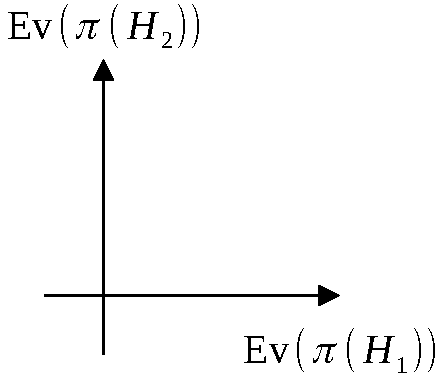
\includegraphics[width=1\linewidth]{images/weights_as_coord.pdf}
	\caption[Weights as coordinates]{Weights as coordinates.}
	\labfig{weigh-as-coord}
\end{marginfigure}
\begin{proposition}
Every representation of $\mathfrak{sl}(3,\mathbb{C})$ has \textbf{at least one weight}.
\end{proposition}
\begin{proof}
As $V$ is a \underline{\textbf{complex}} vector space, $\pi(H_1)$ has at least one eigenvector $v\in V$, i.e. \[
\pi(H_1)v=m_1v\]
Let $\ker(\pi(H_1)^m-\mathbb{1})=:W$. As $\pi(H_2)$ \underline{\textbf{commutes}} with $\pi(H_1)$, then $W$ is invariant under the action of $\pi(H_2)$. So
\[
\pi(H_2)\Bigr|_{\substack{W}}:W\xrightarrow[]{}W
\]
As $W$ is a \underline{\textbf{complex}} linear space, it exists at least an eigenvector\\
$w\neq0,w\in W$ such that:
\[
\begin{cases}
\pi(H_1)w=m_1w\\
\pi(H_2)w=m_2w
\end{cases}
\Rightarrow w\neq0 \text{ is a \textbf{weight vector} with } \mu=(m_1,m_2)
\]
\end{proof}
\begin{proposition}
If $\mu=(m_1,m_2)$ is a weight for a representation
\[
\pi:\mathfrak{sl}(3,\mathbb{C})\xrightarrow[]{}\text{End}(V)
\]
then \textbf{both} $m_1$ \textbf{and} $m_2$ \textbf{are} \textbf{integer numbers}.
\end{proposition}
\begin{proof} (Sketch) 
Consider $\pi$ restricted to:
\[
\begin{cases}
W_1=\text{Span}\{\pi(H_1),\pi(X_1),\pi(Y_1)\}\underset{\textrm{Lie}}{\cong}\mathfrak{sl}(2,\mathbb{C})\\
W_2=\text{Span}\{\pi(H_2),\pi(X_2),\pi(Y_2)\}\underset{\textrm{Lie}}{\cong}\mathfrak{sl}(2,\mathbb{C})
\end{cases}
\]
By the theory of $\mathfrak{sl}(2,\mathbb{C})$ [\refch{RTsl2c}], the eigenvalues of $\pi(H_j)$ should be \textbf{integer}. Hence, both $m_j\in\mathbb{Z}$.
\end{proof}
%1:31:00
\underline{\textbf{Strategy:}} start with a weight vector $v\xleftrightarrow[]{}\mu=(m_1,m_2)$ and "move it"
with $\pi(X_j)$ and $\pi(Y_j)$.
\begin{marginfigure}
    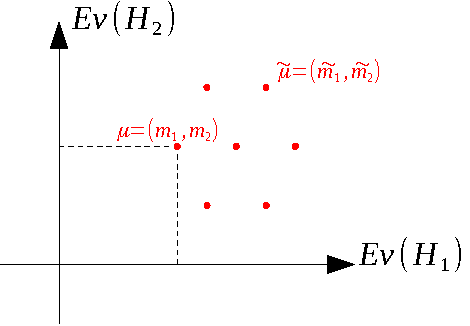
\includegraphics{images/weight_proof_sketch.pdf}
    \caption*{}
    \labfig{weight_proof_sketch}
\end{marginfigure}
\begin{definition}[Roots]\index{Roots}
A pair $\alpha=(\alpha_1,\alpha_2)\in\mathbb{C}^2$ is a \textbf{root} if:
\begin{enumerate}
    \item $(\alpha_1,\alpha_2)\nequiv(0,0)$
    \item $\exists\; Z\in\mathfrak{sl}(3,\mathbb{C}), Z\neq0: \begin{cases}
    [H_1,Z]=\alpha_1 Z\\
    [H_2,Z]=\alpha_2 Z
    \end{cases}
    \quad Z \text{ is the \textbf{root vector}}$
\end{enumerate}
\end{definition}
\begin{kaobox}[frametitle=Remark]
Rewrite the last equation with $ad_X(Y)=[X,Y]$:
\[
\begin{cases}
ad_{H_1}(Z)=\alpha_1 Z\\
ad_{H_2}(Z)=\alpha_2 Z
\end{cases}
\quad Z\neq 0 \;\text{ is a \textbf{simultaneous eigenvector}}
\]
of $ad_{H_1}$ and $ad_{H_1}$. The \textbf{Roots} are \textbf{non-zero weights in the adjoint representation} $\mathfrak{g}\ni x\mapsto ad_x\in\textrm{End}(\mathfrak{g})$.
\end{kaobox}
From the table of commutation relations (cf. \sidecite{Hall2015_Ch4})
\begin{table}[h!]
    \centering
    \begin{tabular}{c|c}
       \hline
       $z$  & $\alpha=(a_1,a_2)$\\
       \hline\hline
       $X_1$ & (+2,-1)\\
       $X_2$ & (-1,+2)\\
       $X_3$ & (+1,+1)
    \end{tabular}
    \qquad 
    \begin{tabular}{c|c}
       \hline
       $z$  & $\alpha=(a_1,a_2)$\\
       \hline\hline
       $Y_1$ & (-2,+1)\\
       $Y_2$ & (+1,-2)\\
       $Y_3$ & (-1,-1)
    \end{tabular}
    \caption{Table of commutation relations.}
    \labtab{roots}
\end{table}
\begin{figure}[h!]
    \centering
    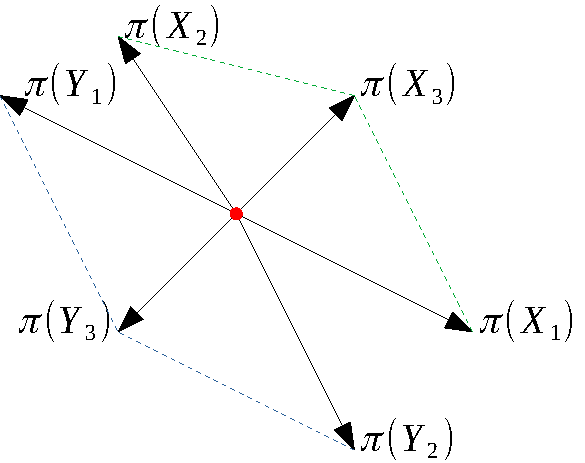
\includegraphics{images/commrelations.pdf}
    \caption*{}
    \labfig{commrelations}
\end{figure}

%INIZIO LEZIONE 25 del 03/06 [Da sentire la registrazione]
\underline{\textbf{Interpretation:}} we say that the weights are "locators" and the roots are "movements", not in a strict sense. 

We can find an analogy with $\mathfrak{sl}(2,\mathbb{C})$:
\begin{figure}[h!]
    \centering
    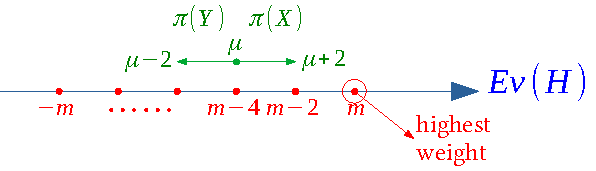
\includegraphics{images/highestweight.pdf}
    \caption{Representation of the case in $\mathfrak{sl}(2,\mathbb{C})$.}
    \labfig{sl(2,C)}
\end{figure}
$\pi(H)$ tells us where we are while how we move on the set is determined by the roots $\pi(x)$ and $\pi(y)$. If we are instead in $\mathfrak{sl}(3,\mathbb{C})$ we are in a two-dimensional plane and we do not have points but pairs.
\begin{figure}[h!]
    \centering
    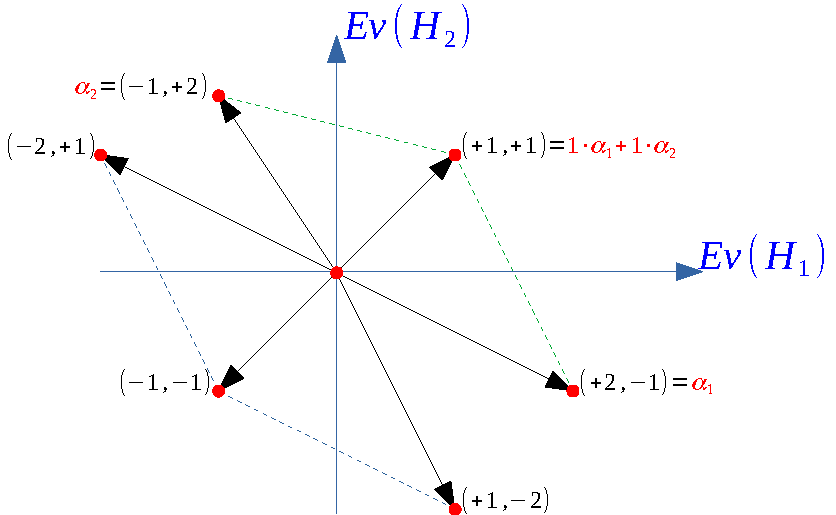
\includegraphics{images/case_sl(3,C).pdf}
    \caption{Representation of the case in $\mathfrak{sl}(3,\mathbb{C})$.}
    \labfig{sl(3,C)}
\end{figure}
\begin{lemma}[Multi-ladder structure]\index{Multi-latter structure}
Let $\alpha=(\alpha_1,\alpha_2)\in\mathbb{C}^2$ be a root and $Z$ the corresponding root vector. Let $\mu=(m_1,m_2)$ be a weight and $v\neq0$ its weight vector:\marginnote{$v$ corresponds to $\mu=(m_1,m_2)$}
\[
\begin{cases}
\pi(H_1)\pi(Z_\alpha)v=(m_1+\alpha_1)\pi(Z_\alpha)v\\
\pi(H_2)\pi(Z_\alpha)v=(m_2+\alpha_2)\pi(Z_\alpha)v
\end{cases}
\]
Hence, \underline{either} $\pi(Z_\alpha)v=0$ \underline{or} $\pi(Z_\alpha)v$ is a (new) weight vector with \textbf{weight} {\color{red}$\mu+\alpha$}
\[
\mu+\alpha=(m_1+\alpha_1,m_2+\alpha_2)
\]
\end{lemma}
\begin{proof}
\begin{align*}
    \pi(H_1)\pi(Z_\alpha)v&=\pi(Z_\alpha)\underbrace{\pi(H_1)v}_{{\color{red}m_1v}}+[\pi(H_1),\pi(Z_\alpha)]v=\\
    &=m_1\pi(Z_\alpha)v+\pi(\underbrace{[H_1,Z_\alpha]}_{{\color{red}\alpha_1Z_\alpha}})v=\\
    &={\color{red}(m_1+\alpha_1)}\pi(Z_\alpha)v
\end{align*}
Similarly, for $\pi(H_2)$ we find the same result with $(m_2+\alpha_2)$ instead.
\end{proof}
\section{The highest weight theory}
\underline{\textbf{Hp:}} Let $\alpha_1=(2,-1)$ and $\alpha_2=(-1,2)$.
\begin{definition}
Let $\mu_1$ and $\mu_2$ be weights. Then $\mu_1$ is \textbf{higher} than $\mu_2$ if $\mu_1-\mu_2$ can be written as:
\[
\mu_1-\mu_2=a\alpha_1+b\alpha_2
\]
with $a,b\ge0$. We write $\mu_1\succeq\mu_2$
\end{definition}
\begin{example}
\[
\left\{
\begin{aligned}
(+1,+1)&=+\alpha_1+\alpha_2\xrightarrow[]{}(+1,+1)\succeq(0,0)\\
(-1,-1)&=-\alpha_1-\alpha_2\xrightarrow[]{}(-1,-1)\preceq(0,0)
\end{aligned}
\right.
\]
\end{example}
\begin{definition}[Highest weight]\index{Highest weight}
A weight $\mu_*$ for $\pi$ is called \underline{a} \textbf{highest weight} if $\mu_*\succeq\mu$ for every weight $\mu$.
\end{definition}
\begin{theorem}[Highest weight theorem]\index{Highest weight theorem}
\begin{enumerate}
    \item Every irreps of $\mathfrak{sl}(3,\mathbb{C})$ is the \textbf{direct sum of the weighted spaces}, (where a weight space for $\mu$ is the linear space generated by weight vectors for $\mu$).
    \[
    V=\bigoplus_{\mu\in\textrm{Weights}(\pi)}\overset{\mathclap{\tikz \node {$\downarrow$} node [above=1.25ex] {\footnotesize Weight space for $\mu$};}}{W_\mu}
    \]
    \item Every irreps $\pi$ has a \underline{\textbf{unique}} \textbf{highest weight}
    \item Two $\textrm{Irreps}(\mathfrak{sl}(3,\mathbb{C}))$, say $\pi_1$ and $\pi_2$, are equivalent if and only if they have the \textbf{same highest weight}
    \item The highest weight of a irreducible representation $\pi$ of $\mathfrak{sl}(3,\mathbb{C})$ has the form {\color{red}$\mu=(m_1,m_2)$} with {\color{red}$m_1,m_2\in\mathbb{N}$}
    \item For every $\mu=(m_1,m_2)\in\mathbb{N}\times\mathbb{N}$ there exists $\pi\in\textrm{irreps}(\mathfrak{sl}(3,\mathbb{C}))$ with highest weight $\mu=(m_1,m_2)$.
\end{enumerate}
\end{theorem}
We are going to prove just Property 5.:
\begin{proof}
\renewcommand{\labelenumi}{0.}
\begin{enumerate}
    \item  $\mu=(0,0)$ is the highest weight for the \textbf{trivial representation}, i.e. $\pi(x)=0 \quad \forall x\in\mathfrak{sl}(3,\mathbb{C})$
\end{enumerate}
\renewcommand{\labelenumi}{\arabic{enumi}.}
\begin{enumerate}
    \item Take now $\mu=(1,0)$: this is the highest weight for the \textbf{fundamental representation}, $\mathfrak{sl}(3,\mathbb{C})\subseteq\textrm{End}(\mathbb{C}^3)$, $\pi(Z)=Z$. We identify the weight vectors with:
\[
\left\{
\begin{aligned}
e_1&=(+1,0)\xleftarrow[]{}{\color{red}\text{highest weight}}\\
e_2&=(-1,+1)\\
e_3&=(0,-1)
\end{aligned}
\right.
\]
For the \textbf{dual representation} $\mathfrak{sl}(3,\mathbb{C})\to\textrm{End}(\mathbb{C}^3)$, i.e. $\pi(Z)={\color{red}-Z^T}$, the weight vectors are given by:
\[
\left\{
\begin{aligned}
e_1&=(-1,0)\\
e_2&=(+1,-1)\\
e_3&=(0,+1)\xleftarrow[]{}{\color{red}\text{highest weight}}
\end{aligned}
\right.
\]
\item Tensor products: $(\pi,V_1)$ is the fundamental representation, $(\pi_2,V_2)$ is the dual representation. We can define:
\[
\pi_{1,1}:\mathfrak{sl}(3,\mathbb{C})\xrightarrow[]{}\text{End}(V_1\otimes V_2)
\]
given by
\[
\pi_{1,1}(X)=(\pi_1\otimes\pi_2)(X)=\pi_1(X)\otimes\mathbb{1}+\mathbb{1}\otimes\pi_2(X) \qquad \Big|\Big|\quad \star
\]
There is a strong analogy with Quantum Mechanics: we take the time evolution in $\mathcal{H}_1$ as $U_1(t)=e^{-itH_1}$ and in $\mathcal{H}_2$ as $U_2(t)=e^{-itH_2}$. In $\mathcal{H}_1\otimes\mathcal{H}_2$, the evolution is given by:
\[
U_{1,2}(t)=U_1(t)\otimes U_2(t)=e^{-itH_*} \quad \textrm{with }\; H_*=H_1\otimes\mathbb{1}+\mathbb{1}\otimes H_2
\]
One checks that if we define $v_{1,1}=e_1\otimes e_3$ (the \textbf{two highest weight vectors}), this is a weight vector with weight (+1,+1)=(+1,0)+(0,+1) and that
\[
\pi_{1,1}(X_j)v_{1,1}=0 \quad \forall j\in\{1,2,3\}
\]
Then we can deduce that (+1,+1) is the highest weight for $\pi_{1,1}$. It is not irreducible, but it contains an Irreps with the same highest weight.
\item More tensor products $\begin{cases}
    (\pi_1,V_1) \quad &\textrm{Fund. representation}\\
    (\pi_2,V_2) \quad &\textrm{Dual representation}
\end{cases}$ 

We define a representation $\pi_{m_1,m_2}$ for $m_1,m_2\in\mathbb{N}$. We then set:
\begin{align*}
\pi_{m_1,m_2}&:\mathfrak{sl}(3,\mathbb{C})\xrightarrow[]{}\text{End}(V_{m_1,m_2})\\
V_{m_1,m_2}&=\underbrace{(V_1\otimes V_1\otimes\dots\otimes V_1)}_{m_1 \text{ times}}\otimes\underbrace{(V_2\otimes V_2\otimes\dots\otimes V_2)}_{m_2 \text{ times}}
\end{align*}
At the end, $\pi_{m_1,m_2}(X)$ is given by:
\begin{align*}
\pi_{m_1,m_2}(X)&=\pi_1(X)\otimes\mathbb{1}\otimes\dots\otimes\mathbb{1}+\mathbb{1}\otimes\pi_1\otimes\mathbb{1}\otimes\dots\otimes\mathbb{1}+\dots\\
&+\pi_2(X)\otimes\mathbb{1}\otimes\dots\otimes\mathbb{1}+\dots+\mathbb{1}\otimes\mathbb{1}\otimes\dots\otimes\pi_2(X)
\end{align*}
It is possible to check that 
\[
v_{m_1,m_2}=\overbrace{v_1\otimes\dots\otimes v_1}^{m_1 \textrm{ times}}\otimes \overbrace{v_2\otimes\dots\otimes v_2}^{m_2 \textrm{ times}}
\]with $v_1$ and $v_2$ highest weight vectors for $\pi_1$ and $\pi_2$ is a weight vector with \textbf{highest weight} $(m_1,m_2)$. Again, we cannot move, in the sense that if we apply a \textit{movement} $\pi(X_j)$ to this guy:
\[
\pi(X_j)v_{m_1,m_2}=0 \quad \forall j\in\{1,2,3\}
\]
It contains an irreps of highest weight $(m_1,m_2)$.
\end{enumerate}
\end{proof}
\paragraph{Isospin:}
\[
T_3=\frac{1}{e}\overset{\mathclap{\tikz \node {$\downarrow$} node [above=1.25ex] {\footnotesize charge};}}{Q}-\frac{1}{e}\overset{\mathclap{\tikz \node {$\downarrow$} node [above=1.25ex] {\footnotesize \parbox{1cm}{\centering average charge}};}}{\expval{Q}}
\]
\underline{Family:} $\{n,p\}:\begin{cases}
T_3(n)=-1/2\\
T_3(p)=+1/2
\end{cases}$


\underline{\textbf{Pictures:}}\begin{marginfigure}
    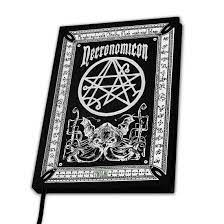
\includegraphics{images/necronomiconvero.jpeg}
\end{marginfigure}
\begin{figure}[h!]
    \centering
    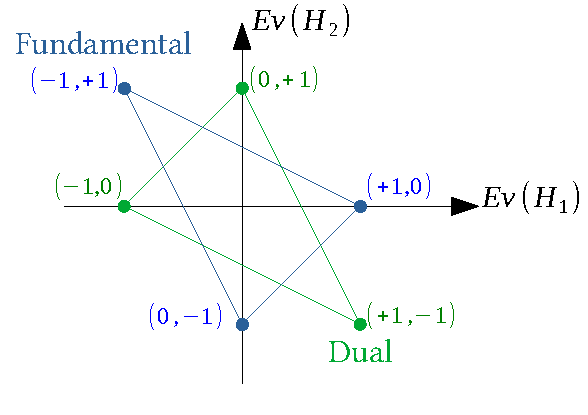
\includegraphics{images/necronomicon.pdf}
    \caption{Clear reference to the \href{https://it.wikipedia.org/wiki/Necronomicon}{Necronomicon} above, you cannot convince me otherwise.}
    \labfig{necronomicon}
\end{figure}
\begin{table}[h!]
    \centering
    \begin{tabular}{c|c}
    \hline
    Fundamental & Dual \\
    \hline\hline
    $\pi(z)=z$ & $\pi(z)=-z^T$ \\
    (+1,0) & (-1,0) \\
    (-1,+1) & (+1,-1) \\
    (0,-1) & (0,1)
    \end{tabular}
    \caption*{}
    \label{tab:my_label}
\end{table}
\section{Cartan subalgebra and Weyl group}
Why did we use $H_1$ and $H_2$? We like the fact that they commute, $[H_1,H_2]=0$ but why not using $H_\pm=\frac{1}{2}(H_1\pm H_2)$? It turns out that what is relevant is the space they generate: $\mathfrak{h}=$Span$_{\mathbb{C}}\{H_1,H_2\}$ is a \textbf{maximal commutative subalgebra} called the \textbf{Cartan subalgebra}.

\raisebox{-\mydepth}{{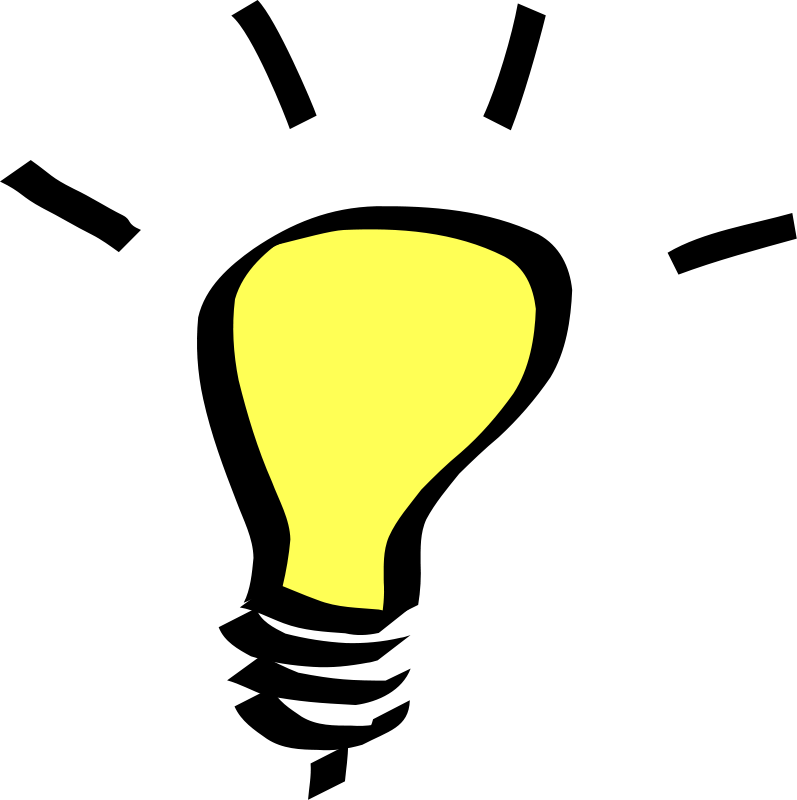
\includegraphics[height=1.1\baselineskip]{images/lamp.png}}} \underline{\textbf{Idea:}} representations of $\mathfrak{sl}(3,\mathbb{C})$ are "\textbf{invariant}" under the \textbf{adjont action} of $\textrm{SU}(3)$. Let $A\in\textrm{SU}(3)$:
\[
\pi_{\color{red}A}(X)=\pi({\color{red}A}X{\color{red}A^{-1}})
\]
In general, $Ad_A(x)=AXA^{-1}$ does \underline{\textbf{not}} preserve the Cartan subalgebra! However, for \underline{\textbf{some}} \textbf{elements} {\color{red}$A\in\textrm{SU}(3)$} it happens that $Ad_A$ preserves $\mathfrak{h}$.
\begin{definition} Let $Z$ and $N$ be:\marginnote{$\mathfrak{h}$ is a Cartan subalgebra

$Ad_{A}$ is the adjoint action}
\[
\begin{split}
Z&=\{A\in\text{SU(3)}:Ad_A(H)=H \quad \forall H\in\mathfrak{h}\}\\
N&=\{A\in\text{SU(3)}:Ad_A(H)\in\mathfrak{h} \quad \forall H\in\mathfrak{h}\}
\end{split}
\]
We have that $Z\subseteq N$
\end{definition}
\begin{proposition}
$Z\trianglelefteq N$\marginnote{$\trianglelefteq$ means "is a \textbf{normal} subgroup of"}
\end{proposition}
\begin{proof} $Z\leq N$ is ok. Now we have to prove that it is normal. Consider $A\in Z$ and $B\in N$, we want to check if it is true that $BAB^{-1}\overset{?}{\in}Z$
\begin{align*}
Ad_{BAB^{-1}}&=\left(BAB^{-1}\right)H\left(BAB^{-1}\right)^{-1}=\\
&=B\overbrace{A\underbrace{B^{-1}HB}_{\mathfrak{h}}A^{-1}}^{Ad_A(\dots)}B^{-1}=\\
&=BB^{-1}HBB^{-1}=\\
&=H
\end{align*}
\end{proof}
% INIZIO L26 del 09/06/2022
This proposition is relevant because, if we have a normal subgroup, the quotient is not only defined as a set, but it is a group itself. Therefore we define:
\begin{definition}[Weyl group]\index{Weyl group}\labdef{weyl-group}
The \textbf{Weyl group} of SU(3), denoted $W$, is the\textbf{ quotient group}
\[
W=N/Z
\]
Where $N$ leaves invariant the Cartan subalgebra $\mathfrak{h}$ as a whole, while $Z$ leaves \textbf{each element} of $\mathfrak{h}$ invariant (it does not move the point at all)
\end{definition}\marginnote[-10mm]{So it is the group of symmetries of our system of weights and roots. Therefore, in a sense, is a second order symmetries: symmetries of the waze of our representation of the algebra of symmetries.}This definition seems artificial, but it is actually very important, especially for elementary particle physics. The \refdef{weyl-group} is rather abstract, we gave it because actually this is the same which works for any semi-simple Lie algebra, provided that it can be defined the Cartan's subalgebras. In our case, we can see it more concretely.
\paragraph{Action of $W$ on $\mathfrak{h}$:} We define an action of $W$ on $\mathfrak{h}$ as follows: for each $w\in W=N/Z$, we choose a representative $A\in N$ so that $[A]=w$. Then, for an arbitrary element of the Cartan subalgebra $H\in\mathfrak{h}$, we set the action of $w$ on $H$ in the most natural way, i.e.
\[
{\color{red}w\cdot H=Ad_{\underset{\mathclap{\tikz \node {$\uparrow$} node [below=1ex] {\footnotesize $A\in N\subseteq \textrm{SU}(3)$};}}{A}}(H)}
\]
We have to check that the action is well-defined, namely that it is independent of the representative. If $\bqty{A}=\bqty{B}\in N/Z$, this means that $A=B \ \textrm{mod}\ Z$, i.e $\exists\;C\in Z:\;B=AC$. We check:
\[
Ad_B(H)=Ad_{AC}(H)\overset{\mathclap{\tikz \node {$\downarrow$} node [above=1.25ex] {\footnotesize The $Ad$ is a group homo};}}{=}Ad_A\underbrace{\left(Ad_C\left(H\right)\right)}_{\underset{\mathclap{\tikz \node {$\uparrow$} node [below=1ex] {\footnotesize $C\in Z$};}}{=}H}=Ad_A(H)
\]
so $Ad_A(H)=Ad_B(H)\quad \forall\;H\in\mathfrak{h}$. \underline{ok}!
\paragraph{Identification:}$W$ is identified with the group of \textbf{linear transformations of} {\color{red}$\mathfrak{h}$} in the form {\color{red}$Ad_A(H)\;\textrm{for}\;A\in N$}, modulo $Ad_C$, where $C\in Z$.\marginnote[-5mm]{We were discussing $\textrm{SU}(3)$ as a guided example, but actually all this part works, more or less the same, for every semi-simple Lie algebra:
\begin{itemize}
    \item Find a Cartan subalgebra inside our semi-simple Lie algebra;
    \item take those elements of the group which leave the algebra invariant by adjoint action;
    \item those other elements of the groups which leave every point of the Cartan subalgebra invariant by the adjoint action
    \item take the quotient: this is the Weyl group.
\end{itemize}}
\begin{proposition}[Explicit form of $N,Z$ and $W$ for $\mathfrak{sl}(3,\mathbb{C})$]\index{Explicit form of $N,Z$ and $W$ for $\mathfrak{sl}(3,\mathbb{C})$}For the special case of $\mathfrak{sl}(3,\mathbb{C})=\textrm{
SU}(3)_{\mathbb{C}}$ we have a concrete representation of $N,Z$ and $W$:
\begin{enumerate}
    \item $Z=\Bqty{\textrm{Diagonal matrices in SU}(3)}=\Bqty{\mqty(\dmat{u_1,u_2,u_1^{-1}u_2^{-1}})}_{u_1,u_2\in \textrm{U}(1)}$
    \item $N$ consists of those $A\in\textrm{SU}(3)$ such that:
    \[
    \forall\;k\in\Bqty{1,2,3}\;\exists\;l=l_k\;\exists\;u_k:
    \quad Ae_k=u_ke_l
    \]
    \item The Weyl group is isomorphic to the \textbf{group of permutations of three elements} $\Bqty{1,2,3}$ or the group of symmetries of \raisebox{-\mydepth}{{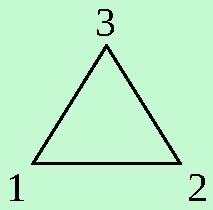
\includegraphics[height=1.5\baselineskip]{images/triangle_verde.pdf}}}\marginnote{$P$ is the number of permutations}
    \[
    \abs{P(3)}=3\cdot 2=6 \quad \textrm{elements}
    \]
\end{enumerate}
\end{proposition}
\begin{proof}
\begin{enumerate}
    \item Suppose $A\in Z$. Then $AHA^{-1}=H\;\;\forall\;H\in\mathfrak{h}$. So $A$ commutes with every element of the Cartan subalgebra, in particular it commutes with $H_1=\textrm{diag}(1,-1,0)$, which has
    \[
    H_1\xrightarrow[]{}
    \begin{cases}
       \textrm{eigenvectors:}\quad & e_1\quad e_2 \quad e_3\\
       \textrm{eigenvalues:}\quad & 1\quad -1\quad 0
    \end{cases}
    \]
    Therefore $A$ must preserve the eigenspaces. But since each one of the eigenvectors is one-dimensional\marginnote{They are one-dimensional because the eigenvalues are all different}, hence
    \[
    AH_1\xrightarrow[]{}\textrm{eigenvectors:} \quad e_1\quad e_2\quad e_3
    \]
    This means that
    \[
    Ae_k={\color{red}\lambda_k}e_k
    \]
    By unitary $(A\in Z\subseteq \textrm{SU}(3))$ $\lambda_k=u_k\in\textrm{U}(1)$, so
    \[
    A=\mqty(\dmat[0]{u_1,u_2,u_3})
    \]
    And since $\det(A)=1$, the third guy is obliged to be $u_3=\left(u_1u_2\right)^{-1}$.
    
    Now we have to check the other direction. Vice versa, every $A$ in the form 
    \[
    A=\mqty(\dmat[0]{u_1,u_2,(u_1u_2)^{-1}})
    \]
    commutes with both $H_1$ and $H_2$\marginnote{It is rather obvious that they commutes because they are both diagonal and diagonal matrices commute with each other}, then $A$ commutes with every linear combination $H=\alpha_1H_1+\alpha_2H_2\in\textrm{Span}_{\mathbb{C}}\Bqty{H_1,H_2}$ which is the Cartan subalgebra $\mathfrak{h}$.
    \item Suppose $A\in N$. Then if we act on $H$ by conjugation we get $AHA^{-1}\in\mathfrak{h}$, which is \textbf{diagonal} and we are still in the Cartan subalgebra.
    \begin{enumerate}
        \item As $H_1=\textrm{diag}(1,-1,0)$ has \textbf{different eigenvalues}, the only possible eigenvectors of
        \[
        AH_1A^{-1}\xrightarrow[]{}
        \begin{cases}
        &Ae_1\quad Ae_2 \quad Ae_3\\
        &1\qquad -1\qquad 0
        \end{cases}
        \]
        Since $AH_1A^{-1}$ is a similarity transformation, we should have the same eigenvalues.
        \item On the other hand, we remind ourselves that $AH_1A^{-1}$ is diagonal, which means
        \[
        AH_1A^{-1}\xrightarrow[]{}
        \begin{cases}
        &e_1\quad e_2 \quad e_3\\
        &\lambda_1\quad \lambda_2\quad \lambda_3
        \end{cases}
        \]
    \end{enumerate}
    Since the claim a) and b) must be both true, the only way is that $\forall\;k\in\Bqty{1,2,3}$
    \[
    \parbox{1.5cm}{$\exists\;l=l(k)$ $\exists\;\lambda_k\in\mathbb{C}$}:\;\; {\color{red}Al_k=\lambda_ke_l}
    \]
    By unitarity, $\lambda_k=u_k\in\textrm{U}(1)$. The vice versa is left as en exercise.
    \item For $k\in\Bqty{1,2,3}$, let $\sigma(k)\in\Bqty{1,2,3}$ such that
    \[
    Ae_k=u_ke_{{\color{red}\sigma(k)}}
    \]
    As {\color{red}$A$} \textbf{is invertible} ($A\in\textrm{SU}(3)$), it cannot be that $\sigma(k)=\sigma(j)$ if $k\neq j$, so we conclude that {\color{red}$\sigma$} \textbf{is a permutation of the set} {\color{red}$\{1,2,3\}$}. More explicitly, every $H\in\mathfrak{h}$ is diagonal
    \[
    H=\mqty(\dmat[0]{\lambda_1,\lambda_2,\lambda_3})
    \]and $AHA^{-1}$ has $e_{\sigma(k)}$ as eigenvector with eigenvalue $\lambda_k$.\marginnote{In a sense, what the Weyl group is doing is permuting the order of the three eigenvalues. Every element of the Cartan subalgebra is diagonal (because it is a linear combination of $H_1$ and $H_2$ which are diagonal), with entries which are complex numbers. Now, the Weyl group, when acting via the adjoint action is permuting them. We could say "ok, but there is much more information than that, because there are also the eigenvalues associated to the element $A$ which are part of the information". \textbf{No}, because we take the quotient via the action of $Z$, which in a sense tells us that the value of the three unimodular numbers (which are two, because the third is constrained by them) is not important.} Notice that although the map we are interested in is $e_k\mapsto {\color{red}u_k}e_{{\color{red}\sigma(k)}}$, the action of $Ad_A{\color{red}\textrm{mod}Z}$ depends only on ${\color{red}\sigma\in\pazocal{P}(3)}$, not on the values $\{u_1,u_2,u_3\}$.
\end{enumerate}
\end{proof}
\subsection{A new viewpoint on weights}
The \refdef{weight-coord-dep} of weights we gave was a simple one for pedagogical reasons, but it is coordinate dependent, so now we will reformulate it. In particular, we saw that $(m_1,m_2)\in\textrm{Ev}(\pi(H_1))\times\textrm{Ev}(\pi(H_2))$, which were our coordinates. This would not be a big problem if the system of coordinates was invariant by action of the Weyl group, but unfortunately it is not.
\begin{marginfigure}
	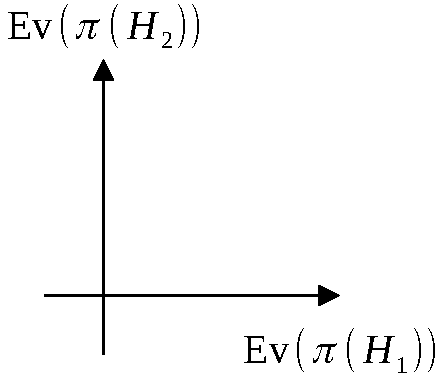
\includegraphics[width=1\linewidth]{images/weights_as_coord.pdf}
	\caption[Weights as coordinates]{Weights as coordinates.}
	\labfig{weigh-as-coord2}
\end{marginfigure}
\[
\text{\parbox{4cm}{{\color{red}{\fontencoding{U}\fontfamily{futs}\selectfont\char 66\relax}}\textbf{This approach is\\coordinate dependent}}}\qquad \text{\parbox{4cm}{{\color{red}{\fontencoding{U}\fontfamily{futs}\selectfont\char 66\relax}}\textbf{The action of the Weyl group does not preserve coordinated $(H_1,H_2)$}}}
\]
Notice that every element of the Cartan subalgebra is a linear combination of the two fundamental ones
\[
\forall\;H\in\mathfrak{h}\qquad H=\alpha_1H_1+\alpha_2H_2
\]
What happens if we take the following?
\[
\pi(\underset{\mathclap{\tikz \node {$\uparrow$} node [below=1ex] {\footnotesize $H\in\mathfrak{h}$ Cartan subalgebra};}}{H})v=\pi\left(\alpha_1H_1+\alpha_2H_2\right)v={\color{red}\;\underbrace{\left(\alpha_1m_1+\alpha_2m_2\right)}_{\text{eigenvalue } \mu(H)}}v
\]
We see that the same $v$ is a simultaneous eigenvector of all $\pi(H)$ as $H$ is varying in the Cartan subalgebra. Moreover we can call this $\mu(H)$, i.e. "the eigenvalue which corresponds to $H$". We have 
\(
{\color{red}\mu:\mathfrak{h}\xrightarrow{\textrm{linear}}\mathbb{C},\;\textrm{i.e.}\; \mu \in\mathfrak{h}^\ast}.
\)
\begin{definition}[Weight - basis indipendent viewpoint]\index{Weight - basis indipendent viewpoint}Let $\mathfrak{h}$ be the Cartan subalgebra, let $\pi:\mathfrak{sl}(3,\mathbb{C})\to\textrm{End}(V)$ be a finite-dimensional representation. A \textbf{linear functional} $\mu\in\mathfrak{h^\ast}$ is called a \textbf{weight for} $\pi$, if $\exists\;v\neq 0,\;v\in V$ such that
\[
\pi(H)v=\mu(H)v 
\]
$\forall\;H\in\mathfrak{h}$.
\end{definition}
The Weyl group $W$ acts linearly on $\mathfrak{h}$, hence it acts on $\mathfrak{h}^\ast$ by setting
\[
\text{\centering\parbox{2cm}{\textbf{Action of} $W$ \textbf{on} $\mathfrak{h}^\ast$}}\quad \Big|\Big|\qquad {\color{red}\left(w\cdot\mu\right)(H):=\mu\left(w^{-1}\cdot H\right)}
\]
Now the interesting point is whether the action of the Weyl group sends a weight into another weight.
\begin{theorem}[Weyl]\index{Weyl's theorem}Suppose $\mu\in\mathfrak{h}^\ast$ is a weight for $\pi\in\textrm{F.D.Rep}(\mathfrak{sl}(3,\mathbb{C}))$. Then, $\forall\;w\in W$
\[
\Big|\Big|\quad w\cdot\mu \;\textrm{ is a weight.}
\]
\end{theorem}
As promised, the Weyl group is a symetry of the set of weights of every representation.
\begin{proof}
$\mu\in\mathfrak{h}^\ast$ is a weight with weight vector $v\neq 0$, by assumption. As $\textrm{SU}(3)$ is \textbf{simply connected}, the representation of the Lie algebra $\pi$ induces a \textbf{Lie \underline{group}} representation 
\[
\begin{split}
\Pi:\textrm{SU}(3)&\to\textrm{GL}(V)\\
A&\mapsto \Pi(A)
\end{split}
\]
We want to see if ${\color{red}\Pi(A)v}$ is a new weight vector. Firs of all, it is different from zero, because the representation $\Pi$ takes values in the general linear group, so invertible endomorphisms.\marginnote{We saw that, when a Lie algebra representation is induced by a Lie group representation, then the adjoint action of the group representation enters in the Lie algebra representation.}
\WithArrowsOptions{displaystyle}
    \[
    \begin{WithArrows}
    \pi(H){\color{red}\Pi(A)v}&=\Pi(A)\overbrace{\Pi(A)^{-1}\pi(H)\Pi(A)}^{\textrm{Adjoint action!}}v=\\
    &=\Pi(A){\color{red}\;\pi(\underbrace{A^{-1}HA}_{\in\mathfrak{h}?})}v=\Arrow{Lemma +\\Assume ${\color{red}A\in N\subseteq\textrm{SU}(3)}$}\\
    &=\Pi(A){\color{red}\;\mu(A^{-1}HA)}v=\Arrow{by linearity}\\
    &={\color{red}\;\mu(A^{-1}HA)}\Pi(A)v
    \end{WithArrows}
    \]
Notice that for ${\color{red}A\in N\subseteq \textrm{SU}(3)}$:
\[
A^{-1}HA=Ad_{A^{-1}}(H)=w^{-1}\cdot H
\]
So the number we got
\[
{\color{red}\mu(A^{-1}HA)=\mu(w^{-1}\cdot H)}\overset{\mathclap{\tikz \node {$\downarrow$} node [above=1.25ex] {\footnotesize By def. of duality};}}{{\color{red}=}}{\color{red}(w\cdot\mu)(H)}
\]
\end{proof}
Summarizing the Weyl group sends a weight into a weight. In a sense, the Weyl group is the group which express the symmetries of the system of weights of our representation.
\subsection{Visualization: coordinate-free viewpoint}
We want to visualize $W\underset{\textrm{"acts on"}}{\hookrightarrow}\mathfrak{h}^\ast$. It is convenient to identify $\mathfrak{h}^\ast$ with $\mathfrak{h}$.%\marginnote{By dimensionality we can always do: for a linear space, the space and the dual have always the same dimension, they are isomorphic. But in general the isomorphism depends on the bases.}
From the theory of Hilbert spaces, we know a natural way to identify a space with the space of linear functionals on it, i.e. every continuous functional on Hilbert space is represented by multiplication tensor vector. So we can do that via an \textbf{Hermitian inner product} on $\mathfrak{h}$. About that, let us recall an important theorem.
\begin{marginfigure}
	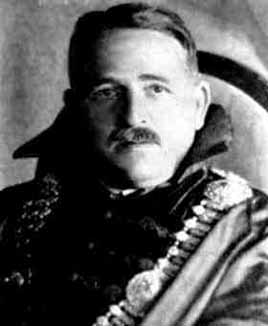
\includegraphics[width=1\linewidth]{images/Frigyes_Riesz.jpeg}
	\caption[Photo of Frigyes Riesz]{From \href{https://commons.wikimedia.org/wiki/File:Frigyes_Riesz.jpeg}{Wikimedia:} Frigyes Riesz (Hungarian: Riesz Frigyes, sometimes spelled as Frederic; 22 January 1880 – 28 February 1956) was a Hungarian mathematician who made fundamental contributions to functional analysis, as did his younger brother Marcel Riesz. He had an uncommon method of giving lectures: he entered the lecture hall with an assistant and a docent. The docent then began reading the proper passages from Riesz's handbook and the assistant wrote the appropriate equations on the blackboard, while Riesz himself stood aside, nodding occasionally.}
	\labfig{Riesz}
\end{marginfigure}
\begin{lemma}[Riesz's lemma]\index{Riesz's lemma}\lablemma{Riesz}Let $\mathcal{H}$ be an Hilbert space. Then for every\footnote{If the Hilbert space is infinite dimensional, $\mathcal{H}^\ast$ means the continuous linear functionals.} $\mu\in\mathcal{H}^\ast\ \exists!\;\psi_\mu\in\mathcal{H}$ such that
\[
\mu(\varphi)=\braket{\psi_\mu}{\varphi}\quad\forall\,\varphi\in\mathcal{H}
\]
\end{lemma}
Hence, we have to equip our $\mathfrak{h}$ with an \textbf{Hermitian inner product} (so that it becomes an Hilbert space and since we are in finite dimension the completeness is automatic): for $H,G\in\mathfrak{h}$, we define
\[
{\color{red}\braket{H}{G}:=\Tr(H^\ast G)}
\]
We check that it is indeed an inner product, $\mathcal{H}$ is complete with respect to the norm and then we can apply Riesz's \reflemma{Riesz}. Also notice that this inner product $\braket{\dots}$ is invariant with respect to the action of $W$: $\forall\,H,K\in\mathfrak{h}\ \forall\,w\in W$
\[
\braket{w\cdot H}{w\cdot K}=\braket{H}{K}
\]
This is essentially because every matrix in the Cartan's subalgebra is diagonal and the Weyl's group acts by permuting the eigenvalues on the diagonal, so the trace will not "feel" that, i.e. as $w$ \textbf{permutes the diagonal entries in $H$.} Therefore, by Riesz's \reflemma{Riesz}, for every $\mu\in\mathfrak{h}^\ast$ \textbf{weight} $\exists!\,\alpha_\mu\in\mathfrak{h}$ such that
\[
{\color{red}\pi(H)v=\langle\underset{\mathclap{\tikz \node {$\uparrow$} node [below=1ex] {\footnotesize Elements of $\mathfrak{h}$};}}{\alpha_\mu}|H\rangle 
v}\;.
\]
Once we have an inner product, we can compute lengths and angles. In particular, we are in the position to compute \textbf{lengths of  weights} $\alpha_\mu\in\mathfrak{h}$ as vectors in the plane and\textbf{ angles among them}. Now there is a part that we skip of \textit{explicit} computations\marginnote{As the professor said, \textit{it is too hot to do this computation}, a not-so-subtle reference to \href{https://www.youtube.com/watch?v=87t3nt5nhZs}{Edoardo Ferrario}: "ma guardi io li potrei pure fà i conti, ma sa qual è il problema? È che oggi fa molto caldo, guardi come stamo messi."} (they are in the book by Hall), but for every weight we can declare that
\[
\norm{\mu}^2=\braket{\alpha_\mu}\qquad \mathfrak{h}^\ast\ni\mu \ \xleftrightarrow{\textrm{Riesz}} \ \alpha_\mu\in\mathfrak{h}
\]
and similarly we can say that\marginnote{It does not happen for every vector that the product is real, but if we take ones which represent weights, then it is ok}
\[
\cos(\mu,\nu)=\frac{\braket{\alpha_\mu}{\alpha_\nu}}{\norm{\mu}\norm{\nu}} \quad \textrm{it happens that} \ \braket{\alpha_\mu}{\alpha_\nu}\in\mathbb{R}
\]
Luckily it happens that the inner product is real, since it is necessary to define the cosine. Now there is a part that we skip of \textit{explicit} computations (they are in Chapter 6 of \sidecite{Hall2015_Ch6}), and we simply give the results.

In \reffig{hall_166} and \reffig{hall_167}, it turns out that, with the Weyl metric, the angles between the roots are $60^\circ$. The right system of coordinates is this sort of \textit{hexagonal paper}.

In \reffig{hall_168}, we draw the dual representation ({\color{Green}green}) and the fundamental one (blue), which were irregular triangles in the naïve representation, but now are equilateral triangles.

In \reffig{hall_169} we take the tensor product of the fundamental and the dual representation. The diagram on top on the left is the $\pi_{(1,1)}$ representation. This is the tensor product of the fundamental and the dual representation, so a priori it has dimension 9, but this tensor product is not irreducible and it decomposes as the direct sum of the representation of dimension 1 and the irreducible representation of dimension 8, which is the one we see in the diagram: $\pi_{(1,1)}$. It has all the weights at the vertex of the hexagon and the center has multiplicity two, hence it has dimension 8 as it should be. Since the movements we are allowed to do are always six, it can be proved that we will always get triangles and hexagons (plus the trivial one, points).
\begin{figure*}[h!]
	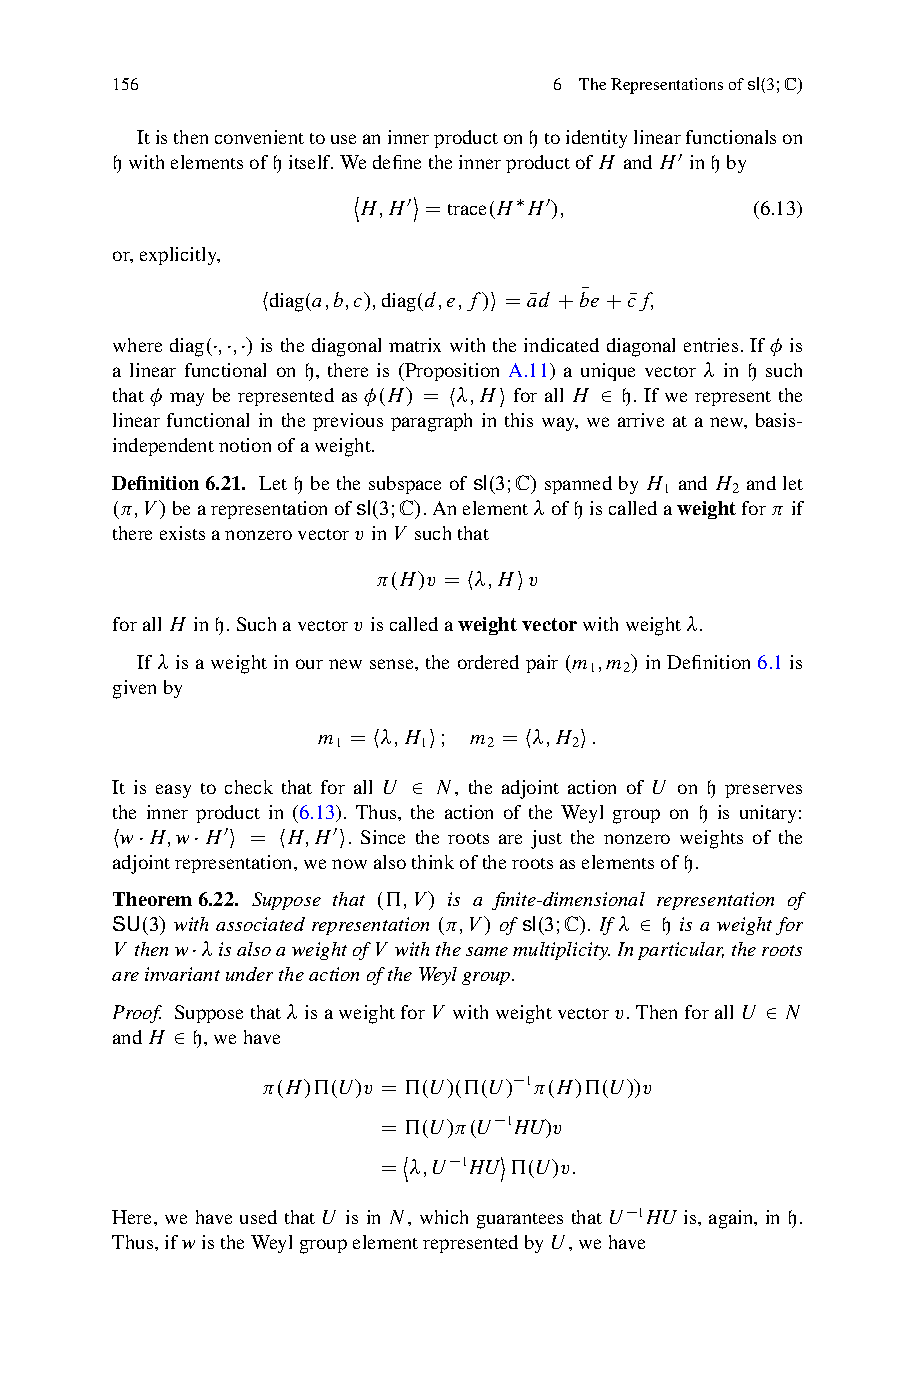
\includegraphics{images/hall_166_c.pdf}
	\caption[]{}
	\labfig{hall_166}
\end{figure*}
\begin{figure*}[h!]
	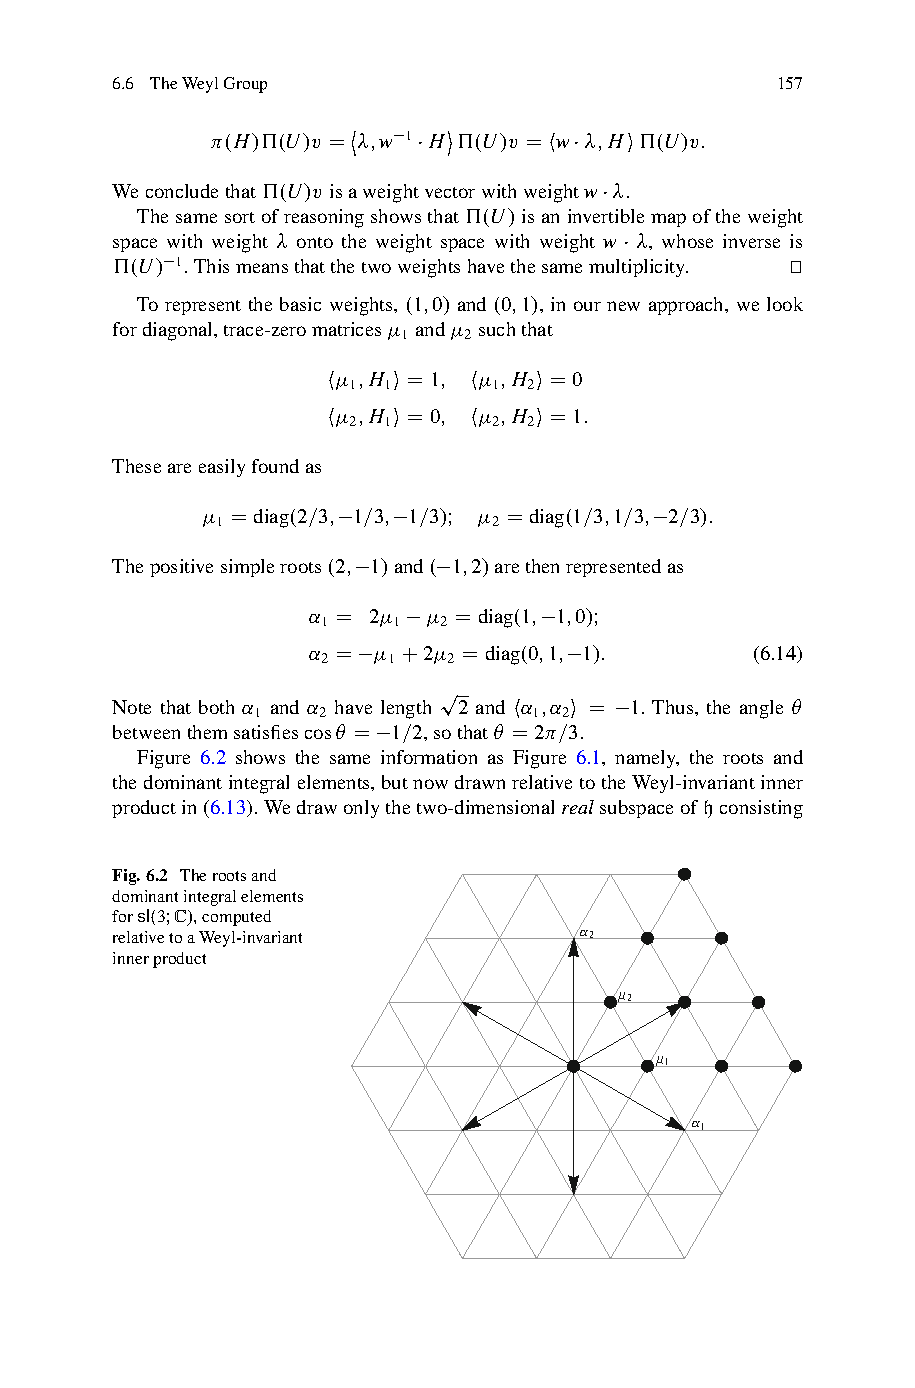
\includegraphics{images/hall_167_c.pdf}
	\caption[]{}
	\labfig{hall_167}
\end{figure*}
\begin{figure*}[h!]
	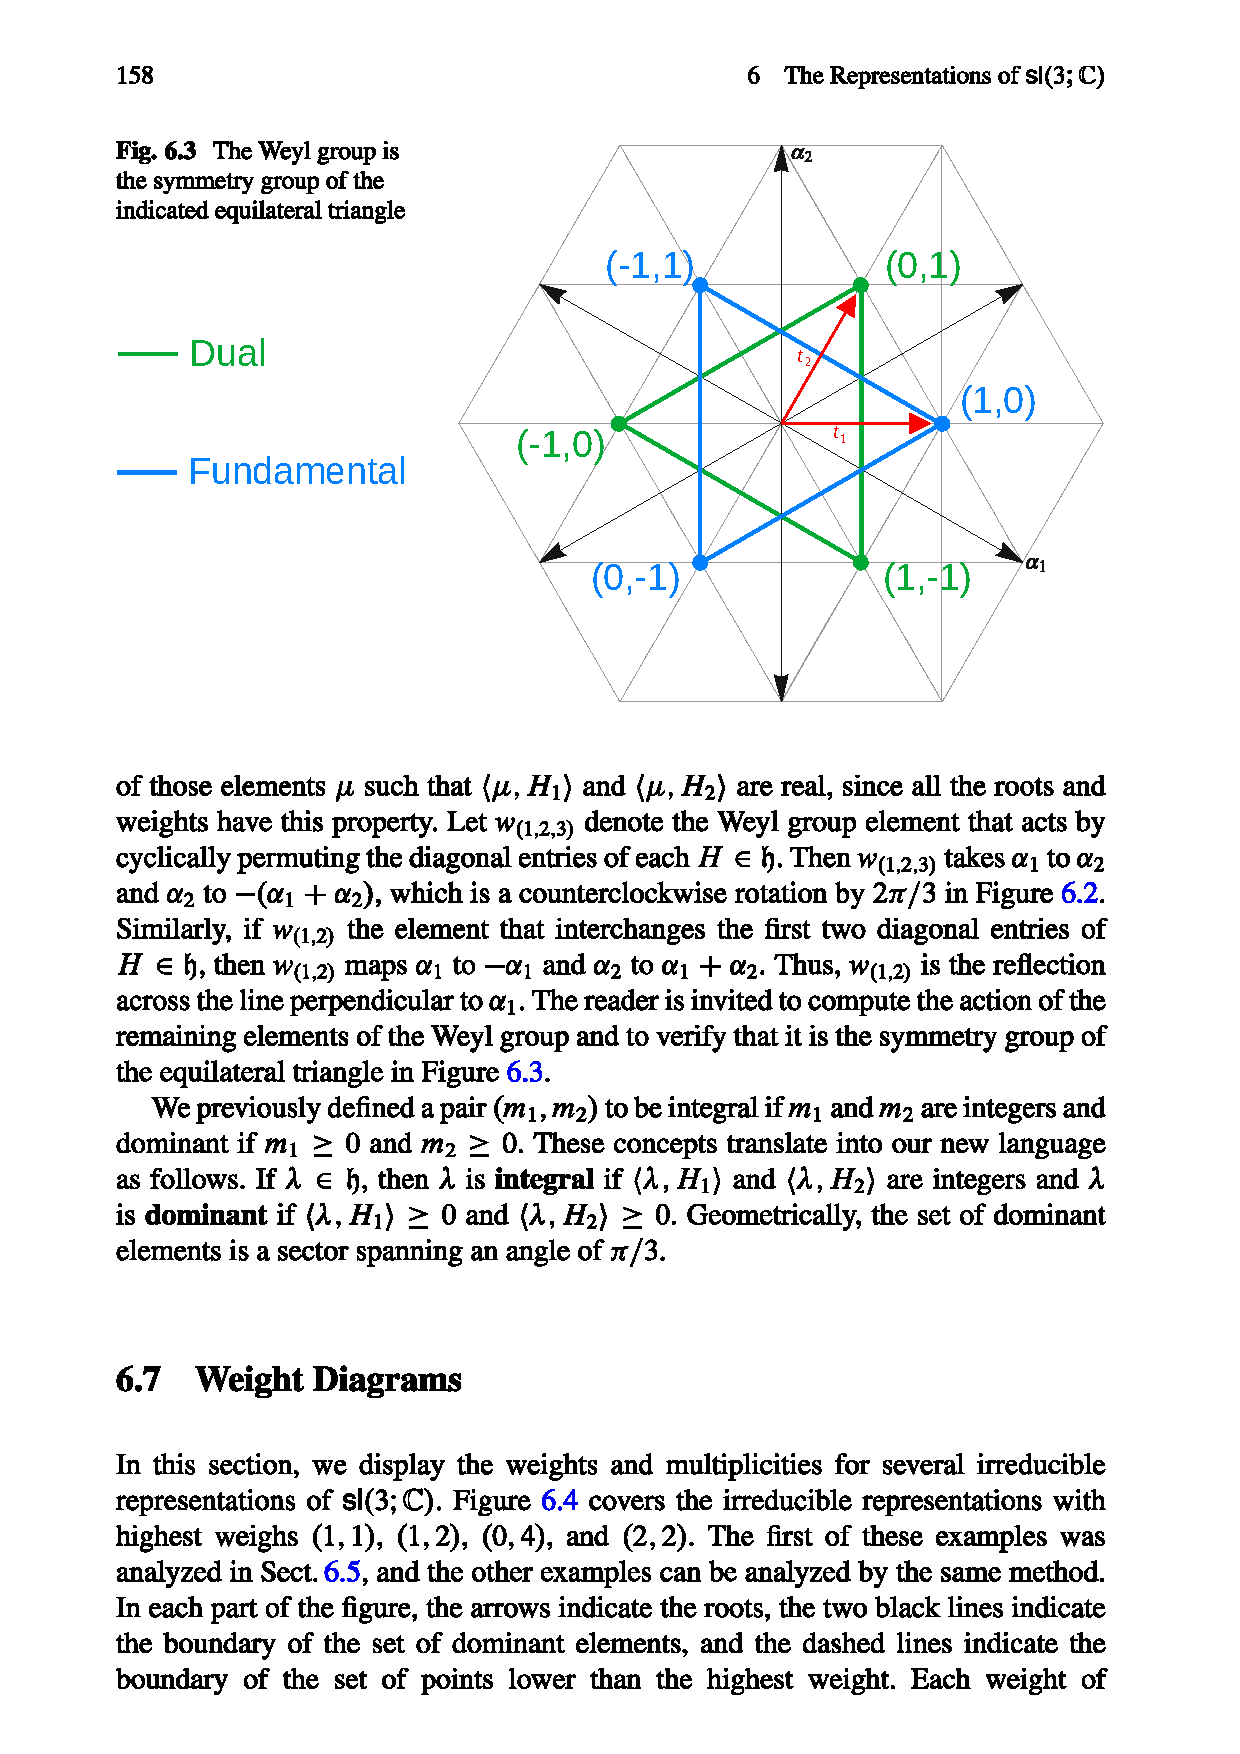
\includegraphics{images/hall_168_c2.pdf}
	\caption[]{}
	\labfig{hall_168}
\end{figure*}
\begin{figure*}[h!]
	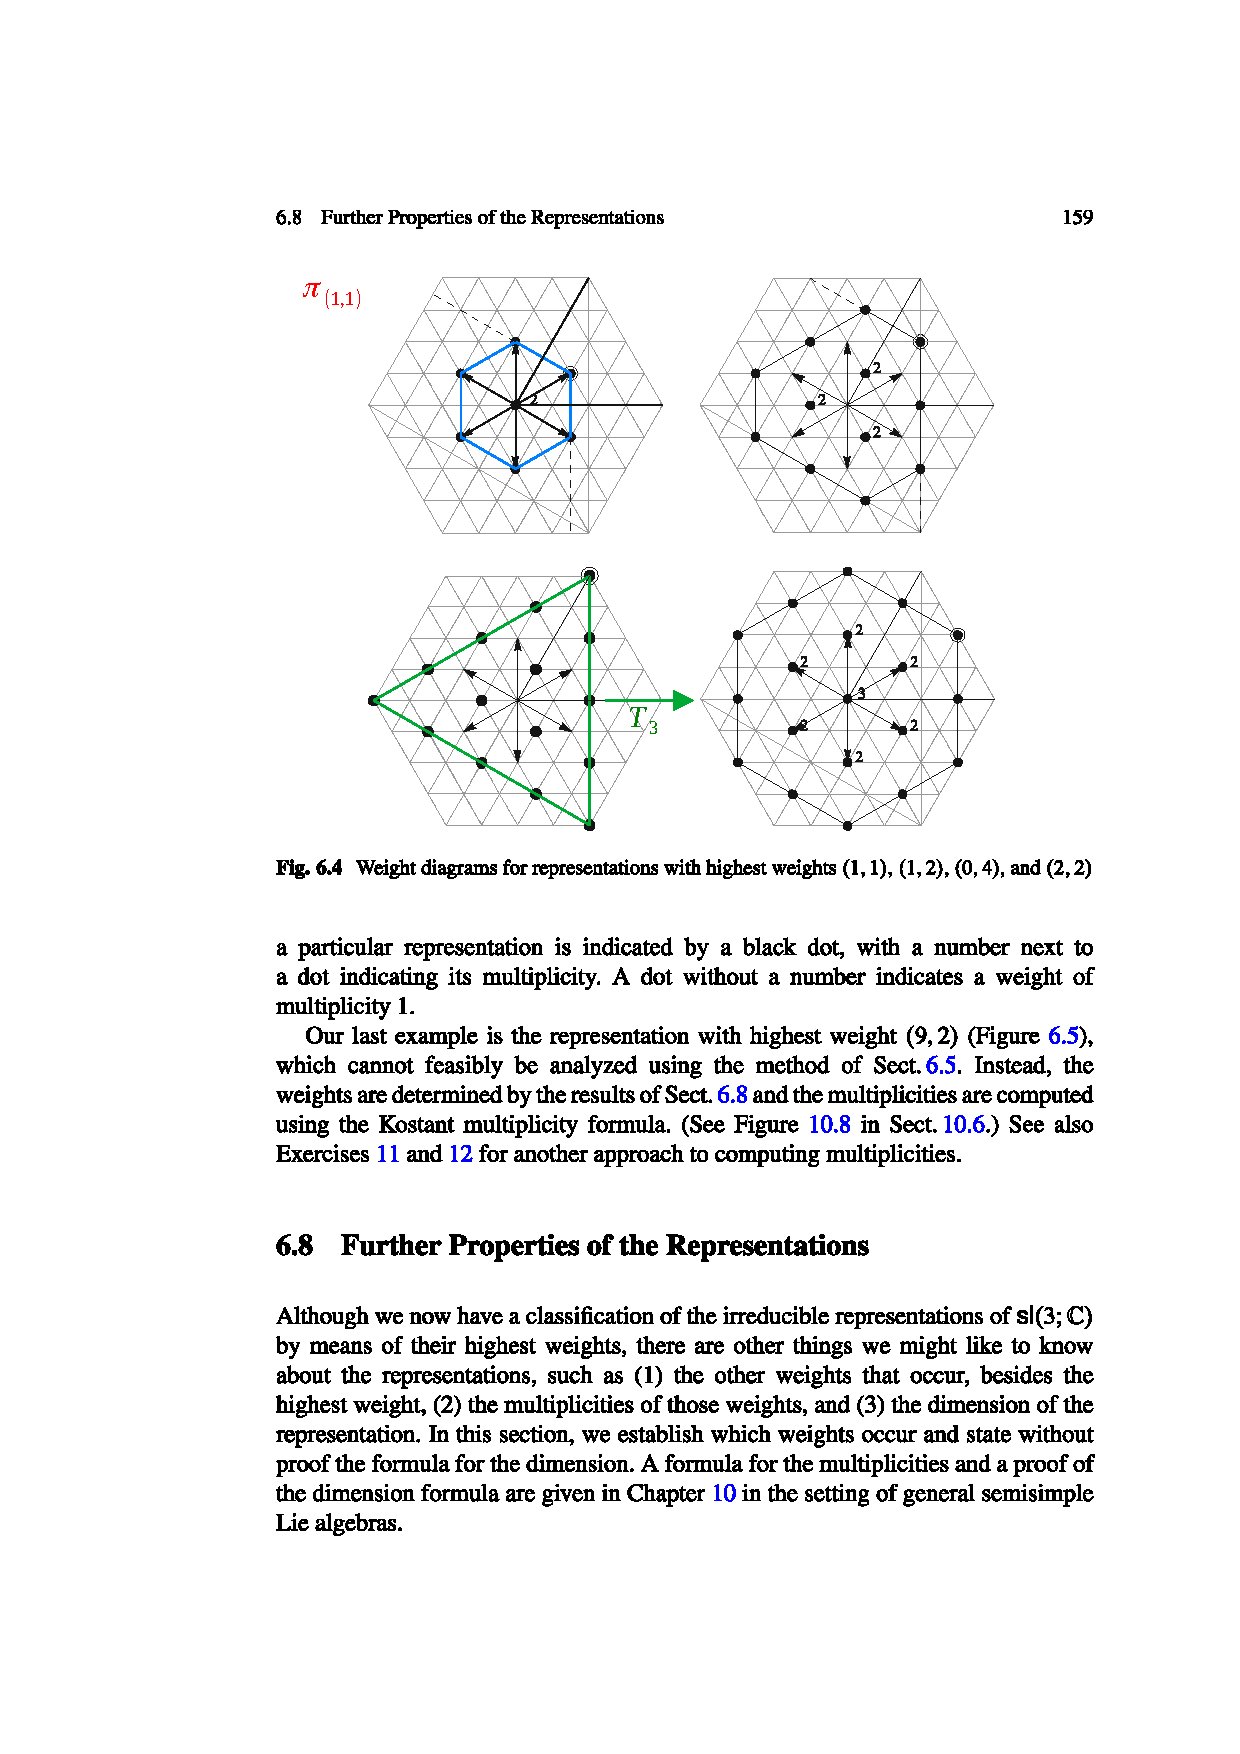
\includegraphics{images/hall_169_c.pdf}
	\caption[]{}
	\labfig{hall_169}
\end{figure*}
Now we apparently change topic, opening a book of nuclear physics \sidecite{krane1988introductory} as in \reffig{krane_733}. We can see that there are hexagons and triangles, but they are a priori completely unrelated, because these are families of elementary particles. We know that elementary particles come in multiplets with similar properties and we classify them according to the isospin and the strangeness. The isospin\index{Isospin} is the difference between the charge of the particle (in natural units) and the average charge of the multiplets. For example, let us focus on the simplest case: the \textit{neutron}\index{neutron} and the \textit{proton}proton. The average charge is $1/2$, therefore the neutron has an excess of $-1/2$ and the proton $+1/2$. \textit{Strangeness}\index{Strangeness} is an artificial quantum number which was introduced to explain why experimentally some possible reactions, among the mesons and barions, were not detected: they would say \textit{if the reaction does not happen, hence the families had different quantum number, different strangeness.} For example we will never see a neutron and a proton to convert themselves into $\Sigma$ particles. $\Sigma$ particles are the one in the lower left diagram and have strangeness $-1$, while neutron and proton have strangeness $0$.
\begin{marginfigure}
	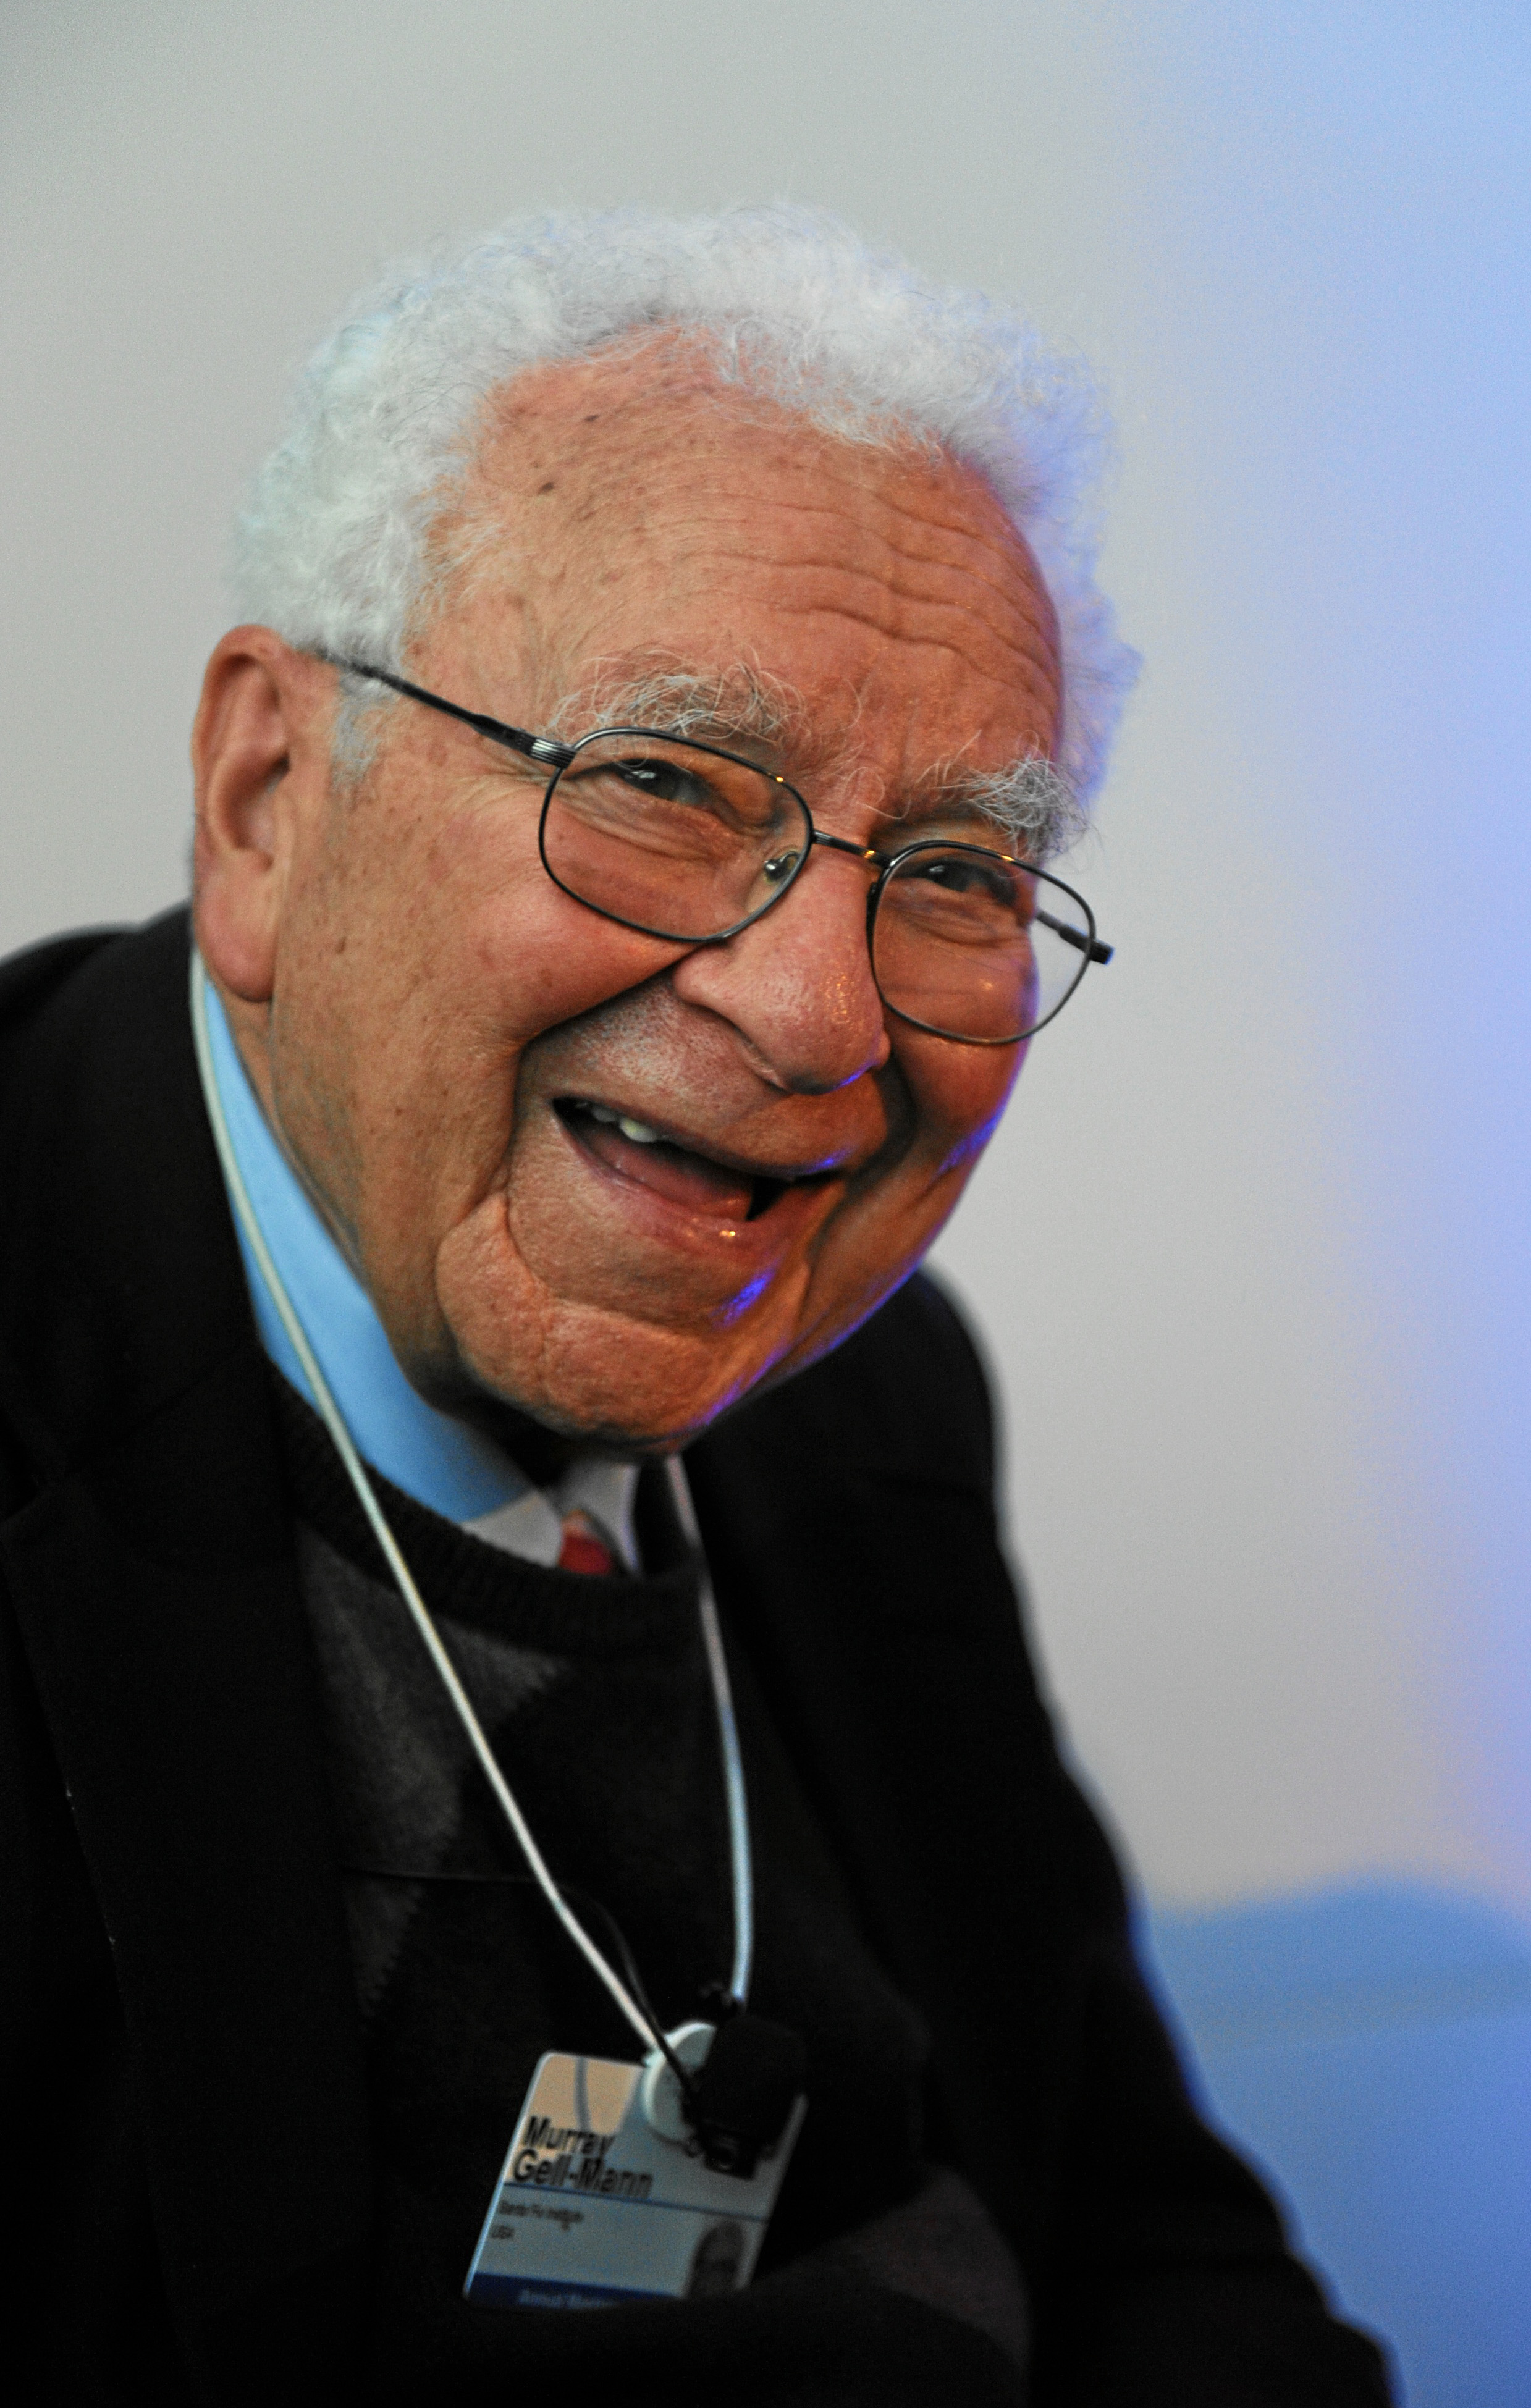
\includegraphics[width=1\linewidth]{images/Murray_Gell-Mann_-_World_Economic_Forum_Annual_Meeting_2012.jpg}
	\caption[Photo of Murray Gell-Mann]{From \href{https://commons.wikimedia.org/wiki/File:Murray_Gell-Mann_-_World_Economic_Forum_Annual_Meeting_2012.jpg}{Wikimedia:} Murray Gell-Mann (September 15, 1929 – May 24, 2019) was an American physicist who received the 1969 Nobel Prize in Physics for his work on the theory of elementary particles. He was the Robert Andrews Millikan Professor of Theoretical Physics Emeritus at the California Institute of Technology, a distinguished fellow and one of the co-founders of the Santa Fe Institute, a professor of physics at the University of New Mexico, and the Presidential Professor of Physics and Medicine at the University of Southern California. Gell-Mann spent several periods at CERN, a nuclear research facility in Switzerland, among others as a John Simon Guggenheim Memorial Foundation fellow in 1972. Gell-Mann died on May 24, 2019, at his home in Santa Fe, New Mexico. }
	\labfig{Gell-Mann}
\end{marginfigure}
\begin{marginfigure}
	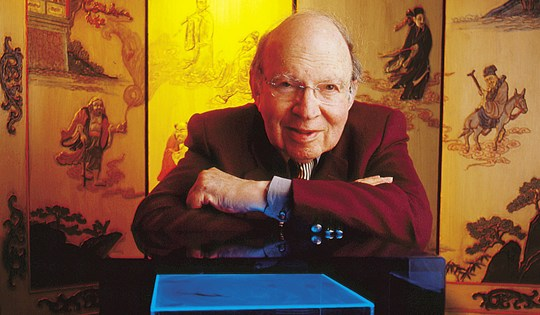
\includegraphics[width=1\linewidth]{images/Yuval_neeman.jpg}
	\caption[Photo of Yuval Ne'eman]{From \href{https://commons.wikimedia.org/wiki/File:Yuval_neeman.jpg}{Wikimedia:} Yuval Ne'eman (14 May 1925 – 26 April 2006) was an Israeli theoretical physicist, military scientist, and politician. He was Minister of Science and Development in the 1980s and early 1990s. He was the President of Tel Aviv University from 1971 to 1977. He was awarded the Israel Prize in the field of exact sciences (which he returned in 1992 in protest of the award of the Israel Prize to Emile Habibi), the Albert Einstein Award, the Wigner Medal, and the EMET Prize for Arts, Sciences and Culture. He died at age 80,[8] on 26 April 2006 in the Ichilov Hospital, Tel Aviv, from a stroke.
	}
	\labfig{Yuval Ne'eman}
\end{marginfigure}
Then, somebody who was well-educated in mathematics, recognised that these diagrams of particles are exactly the weighted diagrams of $\mathfrak{sl}(3,\mathbb{C})$. One of these guy was Gell-Mann and the other was Yuval Ne'eman, who independently developed the theory. They said: "\textit{Look, this is not the fundamental representation, the hexagon is the (1,1) representation, which is an irreducible representation contained in the tensor product of the \textbf{dual and the fundamental} representaion.}". Following Gell-Mann, what we do is supposing that there exists three particles which correspond to the three weights of the fundamental representation, and we give name to them, we call them:
\[
\textrm{\textbf{Up}}, \quad \textrm{\textbf{Down}}, \quad \textrm{\textbf{strange}}
\]
Maybe we can direct them directly, but in a sense every particle we can detect (every meson and barion) is associated to a representation of $\textrm{SU}(3)$, which is obtained by tensorising the fundamental representation and the dual ones (which will be the corresponding anti-quarks). If we tensorize many times, we also obtain triangles. Hence we identify the diagrams of \reffig{krane_733} with the ones of $\mathfrak{sl}(3,\mathbb{C})$. 
\begin{figure*}[h!]
	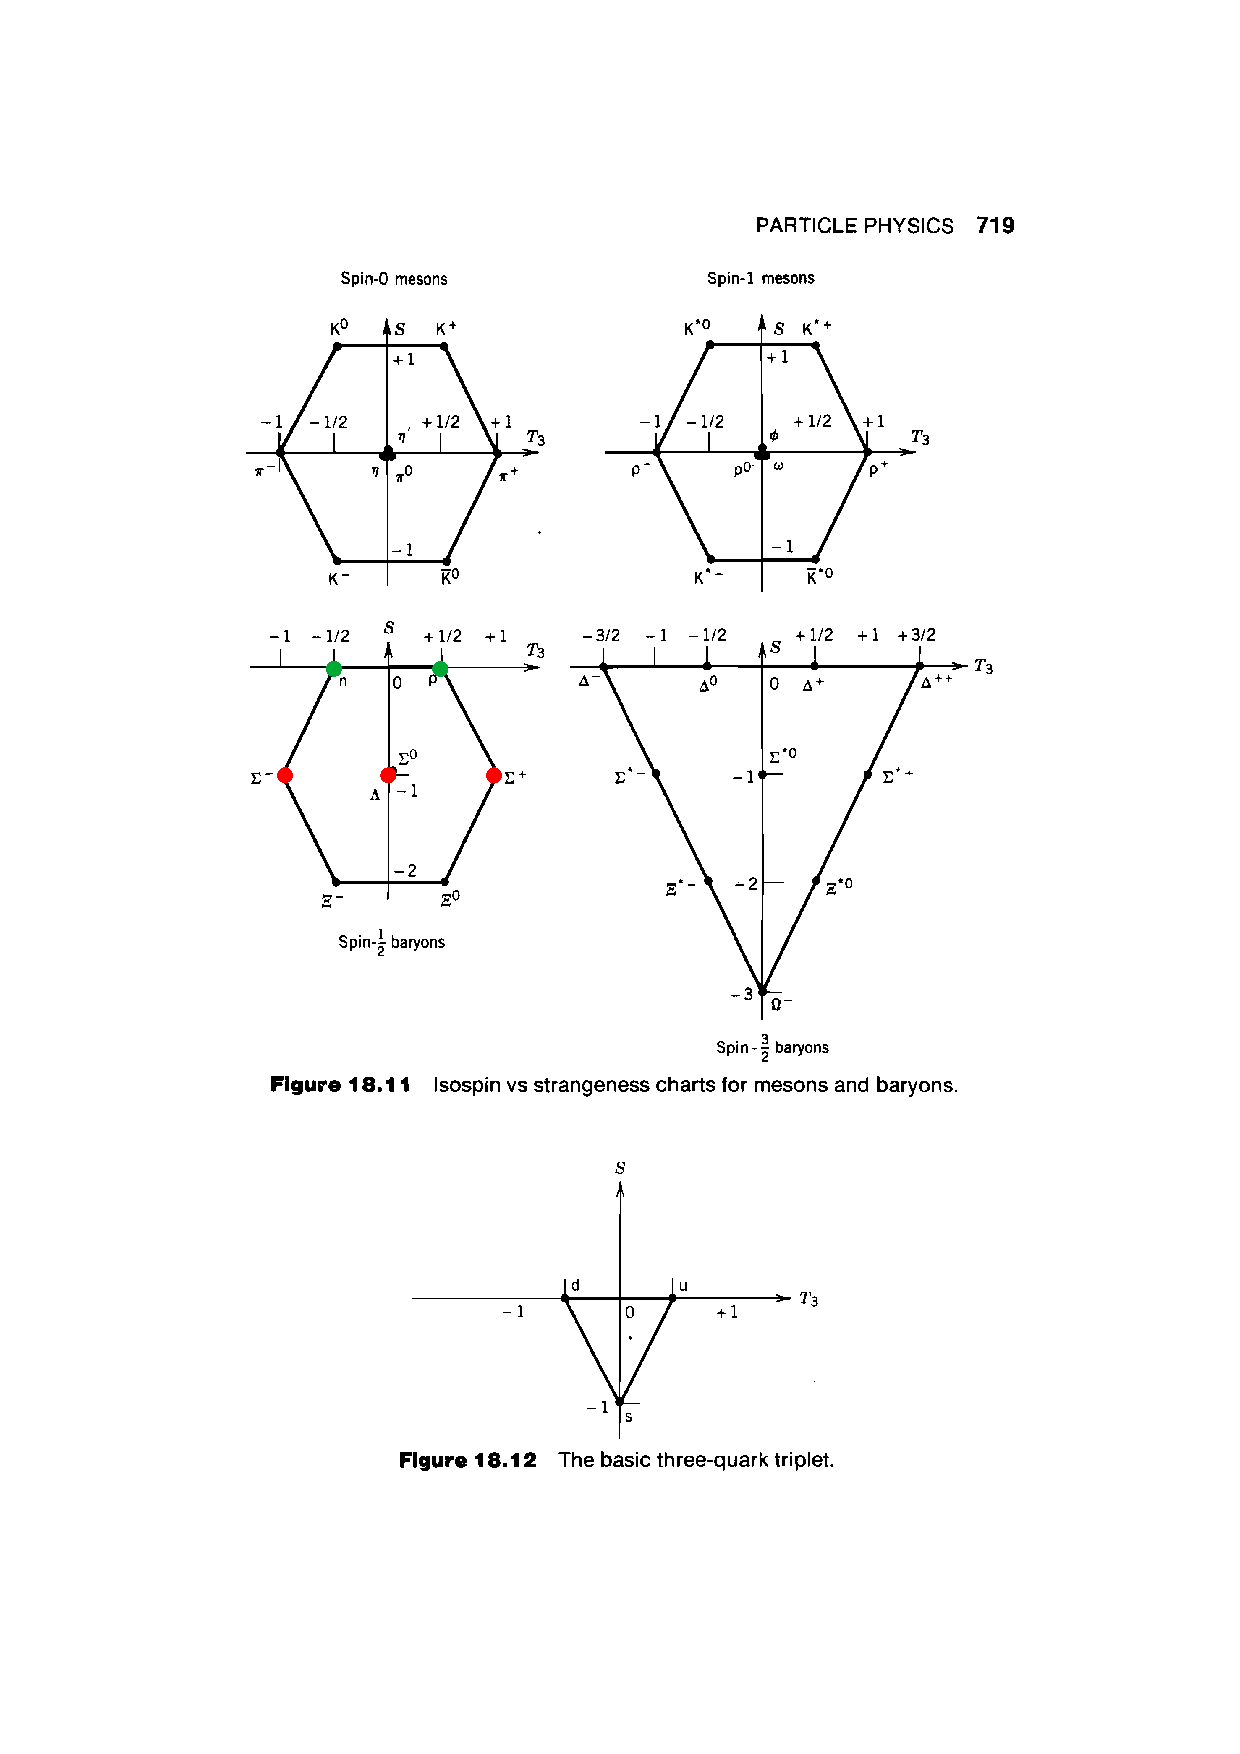
\includegraphics{images/krane_733_c.pdf}
	\caption[]{}
	\labfig{krane_733}
\end{figure*}
\begin{figure*}[h!]
	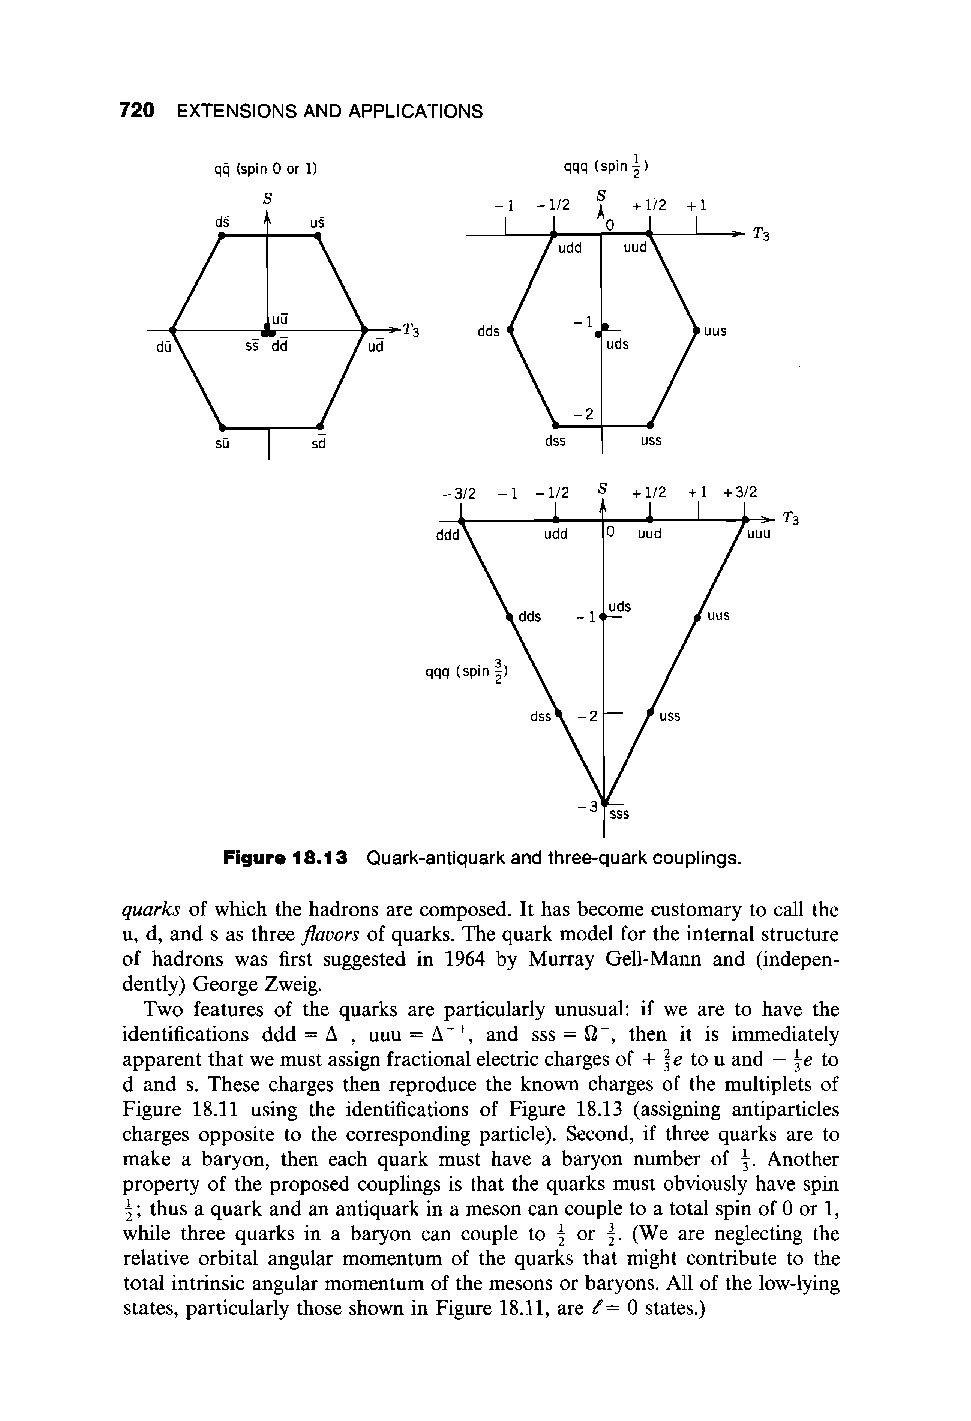
\includegraphics{images/krane-734_c.pdf}
	\caption[]{}
	\labfig{krane_734}
\end{figure*}
In a sense, this is a conceptual viewpoint. What is a particle at the very end? We say that a particle is a relation between the source apparatus and the detector apparatus which obeys some fundamental symmetries of nature. The first and most fundamental symmetry is the one given by the Lorentz group (or Poincaré group) and then there are internal symmetries that these relations have to obey, and these are, in the case of mesons and baryons, the one dictated by $\textrm{SU}(3)$. The question "\textit{Are there particles which really obey the fundamental or the dual representation of $\textrm{SU}(3)$?}" is not well-posed. Because what is important to us is that all the particles we know obey some representation of $\textrm{SU}(3)$. Then we declare that the particles which are the fundamental representation correspond to three mysterious guys. They come in three and, since a popular Bavarian dish is to serve three small piece of cheese (\textit{ricottine} in Italian), which in Bavarian german are called \textbf{quark}.
%1:44:00
\end{document}